\documentclass{article}



\usepackage{amsmath, amsfonts, amsthm} % Math packages

\usepackage{listings} % Code listings, with syntax highlighting

\usepackage[utf8]{inputenc} % Required for inputting international characters
\usepackage[T1]{fontenc} % Use 8-bit encoding

\usepackage[english, greek]{babel} % English language hyphenation
\usepackage{alphabeta}

\usepackage{graphicx} % Required for inserting images
\graphicspath{{Figures/}{./}} % Specifies where to look for included images (trailing slash required)

\usepackage{booktabs} % Required for better horizontal rules in tables

\usepackage{dirtytalk} % Required for quoting.

\usepackage{float} % Added for hard placement of images.

\usepackage[dvipsnames]{xcolor} % Added for extra colors.

\usepackage{tikz} % For colored boxes and more.

\numberwithin{equation}{section} % Number equations within sections (i.e. 1.1, 1.2, 2.1, 2.2 instead of 1, 2, 3, 4)
\numberwithin{figure}{section} % Number figures within sections (i.e. 1.1, 1.2, 2.1, 2.2 instead of 1, 2, 3, 4)
\numberwithin{table}{section} % Number tables within sections (i.e. 1.1, 1.2, 2.1, 2.2 instead of 1, 2, 3, 4)

\usepackage{translator}

\newcommand{\en}[1]{\foreignlanguage{english}{#1}}
\newcommand{\src}[1]{\texttt{\en{#1}}}


% Extra Formatting

\setlength{\parindent}{0em}
\setlength{\parskip}{0em}


% Code Listing Style

\lstdefinestyle{code}{
  belowcaptionskip=1\baselineskip,
  breaklines=true,
  frame=LRTB,
  xleftmargin=\parindent,
  showstringspaces=false,
  basicstyle=\ttfamily,
  keywordstyle=\bfseries\color{green!40!black},
  commentstyle=\itshape\color{purple!40!black},
  identifierstyle=\color{black},
  stringstyle=\color{orange},
}


\newcommand{\lstcode}[4][]
{
    \begin{otherlanguage}{english}
        \lstinputlisting[language=#3, frame=single, style=code, caption={#4}, label={#1}]{#2}
    \end{otherlanguage}
}

% Some Greek stuff
\usepackage{graphicx}
\usepackage{indentfirst}
\usepackage{verbatim}
\usepackage{amsmath}
\usepackage{amsthm}
\usepackage{amssymb}
\usepackage{hyphenat}
\usepackage{makeidx}

\addto\captionsgreek{%
  \renewcommand{\indexname}{Ευρετήριο όρων}%
  \renewcommand{\bibname}{\textgreek{Βιβλιογραφία}}%
}

% latin text (and greek text)
\newcommand{\tl}[1]{\textlatin{#1}}
\newcommand{\tg}[1]{\textgreek{#1}}
\newcommand{\lat} {\latintext} 
\newcommand{\gre}{\greektext}


\usepackage{lineno}
\usepackage{hyperref}
\usepackage{cleveref}
\modulolinenumbers[5]

\usetikzlibrary{positioning}

\crefname{equation}{εξ.}{εξ.}

\makeindex

%% `Elsevier LaTeX' style
\bibliographystyle{ieeetr}
%%%%%%%%%%%%%%%%%%%%%%%

\begin{document}

\begin{titlepage}

\title{Σχεδιασμός και υλοποίηση ψηφιακού ισοσταθμιστή ήχου.}
% \tnotetext[mytitlenote]{Fully documented templates are available in the elsarticle package on \href{http://www.ctan.org/tex-archive/macros/latex/contrib/elsarticle}{CTAN}.}

%% Group authors per affiliation:
\author{Ευάγγελος Λάμπρου}
\date{}

\maketitle

\begin{abstract}
    Στα πλαίσια αυτής της εργασίας γίνεται ο σχεδιασμός και υλοποίηση 
    ενός ισοσταθμιστή ήχου. 
\end{abstract}

% \begin{keyword}
%     \en{DSP}\sep \en{plguin}\sep ισοστάθμιση
% % \MSC[2010] 00-01\sep  99-00
% \end{keyword}

\end{titlepage}

\linenumbers

\section{Σχεδιασμός}

\begin{figure}[htpb]

    \begin{center}

        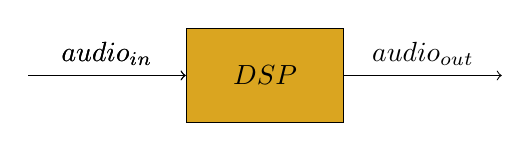
\begin{tikzpicture}

        % \node[draw,
        %     circle,
        %     minimum size=0.6cm,
        %     fill=Rhodamine!50
        %     ] (sum) at (0,0){};
        % \draw (sum.north east) -- (sum.south west)
        %     (sum.north west) -- (sum.south east);
        % \node[left=-1pt] at (sum.center){\tiny $+$};
        % \node[below] at (sum.center){\tiny $-$};

        % Controller

        \node [draw,
        fill=Goldenrod,
        minimum width=2cm,
        minimum height=1.2cm,
        right=1cm
            ] (dsp) {$DSP$};

        \draw[->] ++(-1,0) -- (dsp.west) 
            node[midway,above]{$audio_{in}$};

        \draw[->] ++(-1,0) -- (dsp.west) 
            node[midway,above]{$audio_{in}$};

        \draw[->] (dsp.east) --  ++(+2,0) 
            node[midway,above]{$audio_{out}$};
        \end{tikzpicture}
    \end{center}

    \caption{Βασική δομή του \en{plugin}.} 
\end{figure}

\paragraph{Θεωρία \en{IIR} φίλτρων}

Στην εργασία αυτή θα περιοριστούμε στην υλοποίηση φίλτρων 2ης τάξης, με τους 
αλγόριθμους όμως να είναι ικανούς να παράγουν φίλτρα οσοδήποτε μεγάλης τάξης (χωρίς 
βέβαια να εγγυάται η ορθότητα του τελικού αποτελέσματος λόγω πεπαρασμένης ακρίβειας 
στις τιμές των συντελεστών). 

Έχοντας ως βάση ένα χαμηλοπερατό φίλτρο 2ης τάξης \cite{OpenheimAlan}

\begin{equation}
    H(s) = \frac{1}{s^2 + s/Q + 1} 
    \label{eq:h_lowpassfilter}
\end{equation}

Μέσω του διπολικού $Z$ μετασχηματισμού, θέτωντας $s = 2f_s\frac{z-1}{z+1}$ έχουμε \cite{BilinearZTransformWeb}

\begin{equation}
    H(z) =  
\end{equation}


\paragraph{Φίλτρα \en{Butteworth}} 

\cite{Butteworth1930}

Για τους συντελεστές του φίλτρου \en{Butterworth} μπορούμε απλά να υπολογίσουμε την τιμή 
της σταθεράς $Q$ και να πάρουμε τους συντελεστές από την \cref{eq:h_lowpassfilter} \cite{OpenheimAlan, JuceDocumentation}

\begin{align}
    1/Q &= {2cos(\frac{2i + 1}{n}\pi)}, \; i = 0..\frac{n}{2} \qquad n = {\text{άρτιο}} \\ 
    1/Q &= {2cos(\frac{i + 1}{2n}\pi)}, \; i = 0..\frac{n}{2} \qquad n = {\text{περιττό}}
\end{align}

\paragraph{Αλγόριθμος Υπολογισμού Συντελεστών}

Από την προηγούμενη μαθηματική ανάλυση, ο υπολογισμός των συντελεστών για το εκάστοτε φίλτρο είναι πλέον 
τετριμένος. 


\section{Υλοποίηση}

Για την υλοποίηση του φίλτρου χρησιμοποιήθηκαν οι βιβλιοθήκες του πακέτου 
\en{Juce}. Το πακέτο αυτό χωρίζεται σε ενότητες \en{(modules)}, από τις οποίες
χρησιμοποιούμε κατά βάση την ενότητα \src{juce::dsp}. 
Εδώ, περιλαμβάνονται κλάσεις μέσω την οποίων μπορεί να γίνει η δημιουργία 
ενός φίλτρου.

Ο τρόπος με τον οποίο η εφαρμογή μας επεξεργάζεται τα εισερχόμενα δείγματα
\en{(samples)} είναι στη ρουτίνα \src{processBlock} όπου δεχόμαστε σαν είσοδο έναν
\en{buffer} από δείγματα στα οποία μπορούσαμε να εφαρφμόσουμε οποιονδήποτε αλγόριθμο. 

Το \en{plugin} στην πραγματικότητα αποτελείται από τρία (3) φίλτρα: 

\begin{enumerate}
    \item Ένα χαμηλοπερατό φίλτρο \en{(low pass filter)}
    \item Ένα φίλτρο κορυφής
    \item Ένα υψηπερατό φίλτρο
\end{enumerate}

Ο τρόπος με τον οποίο αυτό περιγράφεται στον κώδικα είναι μέσω της δομής 
\src{ProcessorChain} η οποία αναπαριστά μία αλυσιδά επεξεργαστών. 
Κατά την εκτέλεση της εφαρμογής, η ακολουθία από δείγματα
περνάει από την ρουτίνα επεξεργασίας του κάθε φίλτρου διαδοχικά. \cite{JuceDocumentation}


\paragraph{Γραφική Διεπαφή}
\paragraph{Χρήση}

\begin{figure}[htpb]
    \centering
    \includegraphics[width=0.8\textwidth]{./assets/Carla_Basic.png}
    \caption{Εφαρμογή του \src{SimpleEq plugin} στο περιβάλλον \en{Carla}.}
    \label{fig:carla_basic}
\end{figure}


\paragraph{Μετρήσεις}

Μετά τη δημιουργία της εφαρμογής ισοστάθμισης, έγινε εισαγωγή του \en{plugin} 
\src{SimpleEQ} στο περιβάλλον επεξεργασίας ψηφιακού ήχου (\en{DAW}) \en{Ardour}, 
το οποίο λειτουργεί σαν υποδοχέας και παρέχει δυνατότητες μέτρησης της απόκρισης συχνότας και 
φάσης του φίλτρου (\cref{fig:ardour_analysis}).

\begin{figure}[htpb]
    \centering
    \includegraphics[width=0.8\textwidth]{./assets/PluginAnalysisArdour.png}
    \caption{Ανάλυση του \src{SimpleEQ} μέσα από το \en{Ardour}. Φαίνεται η απόκριση συχνότητας (άσπρο) και η απόκριση φάσης (κόκκινο).}
    \label{fig:ardour_analysis}
\end{figure}

\newpage

\bibliography{bibliography}

\end{document}
